Esta abordagem facilitará aos envolvidos perceberem seus níveis de proficiências e aprofundamentos em determinadas temáticas ou áreas do conhecimento, contribuindo assim para que, em seus processos de escolha de seus Projetos de Vida, sejam mais assertivos tanto na área ou campo de atuação que desejam seguir em suas vidas acadêmicas, principalmente em qual curso, faculdade ou mercado de trabalho possuem maior afinidade para se dedicar. Este processo não exclui a possibilidade de mudança de carreira do indivíduo em determinado momento, onde ele poderá escolher seguir uma outra carreira ou atuar em uma nova área de conhecimento. A intenção deste processo é fazer com que durante a aprendizagem e compreensão de novas possibilidades se torne válida, e não apenas a escolha como opção final, estancada, onde muitas vezes o indivíduo se torna infeliz com as escolhas, sem enxergar a possibilidade das mudanças que poderão ocorrer ao longo do percurso.  
\\

Com foco aos professores, o intuito é incentivá-los à compreensão de novas didáticas e metodologias de ensino, para aplicarem em sala de aula através do Plano de Aula e do Roteiro Pedagógico Gamificado. Assim que os professores conseguirem compreender o processo e se apropriarem da proposta, o ato de fazer o Plano de Aula, no formato do Roteiro Pedagógico Gamificado, se tornará natural, não sendo necessário criar dois documentos separados, mas únicos, envolvendo as Habilidades, Competências e Conteúdos que serão trabalhados durante aquela "Aventura", podendo envolver mais de uma Área de Conhecimento, pois a intenção deste processo é mostrar não somente ao estudante, mas também aos Professores, que a formação integral está nesta esfera.
\\

Não se pode falar sobre Gamificação Pedagógica sem pontuar a necessidade de ter as recompensas e conquistas alcançadas pelos estudantes, possibilitando um maior engajamento na participação e desenvolvimento da aplicação do processo. Estes prêmios podem variar desde elementos estéticos para o personagem selecionado, até bônus reais no desenvolvimento de ações e atividades, assim como no alcance de resultados e conceitos, como em testes de ações dos participantes. No processo, é necessário escolher qual o
"universo" que será utilizado como pano de fundo para a Gamificação, podendo envolver elementos da Segunda Guerra Mundial, do Egito Antigo, do Brasil Colônia, da Revolução Industrial, de Fantasia Medieval, de Ficção Científica, entre outros. O importante é envolver todos os campos e áreas do conhecimento, destacando a necessidade e compreensão do Currículo Transdisciplinar, em que estarão trabalhando não somente a História, mas também a Geografia, Sociologia, Filosofia, Arte, Literatura, Língua Estrangeira Moderna, Matemática, Ciências, Biologia, Física, Química, Tecnologia, Educação Física e Língua Portuguesa, de forma inter, multi e transdisciplinar, mostrando que um componente não pode existir sem se
relacionar em algum grau de aprofundamento com o outro, e desta forma, quebrar o paradigma de que os únicos componentes que são importantes para o desenvolvimento do indivíduo são a Língua Portuguesa e a Matemática.
\\

O Processo se dará em duas etapas: uma de maneira lúdica, com a Gamificação, para que os estudantes possam compreender e desenvolver as Habilidades, Competências e Conteúdos, e depois o firme desta compreensão com a aplicação de atividades estruturadas para conferir se realmente consolidaram estes conhecimentos.

\textbf{OBJETIVOS ESPECÍFICOS}
\\

\begin{itemize}

  \item \textbf{Desenvolvimento de uma Trilha Pedagógica Gamificada com Elementos de RPG:} O principal objetivo é criar uma abordagem pedagógica que integre elementos de Jogos de Interpretação de Papéis (RPG) dentro de metodologias ativas de aprendizagem, aproveitando também a tecnologia educacional para oferecer recursos interativos e engajadores;
\\
  \item \textbf{Integração do Desenho Universal para Aprendizagem (DUA):} Incorporar os princípios do Desenho Universal para Aprendizagem visa garantir a inclusividade e acessibilidade em diversos ambientes acadêmicos, aproveitando a tecnologia para oferecer suporte a diferentes estilos de aprendizagem e necessidades dos estudantes; 
\\
  \item \textbf{Promoção da Educação Integral:} O objetivo é promover uma educação holística alinhada com as metas estabelecidas na Base Nacional Comum Curricular (BNCC, 2018), fazendo uso da tecnologia educacional para enriquecer experiências de aprendizagem e ampliar o acesso a recursos educacionais;
\\
  \item \textbf{Aprimoramento do Significado da Aprendizagem:} Projetar trilhas pedagógicas gamificadas que transcendam fronteiras disciplinares para tornar a aprendizagem mais significativa, integrando tecnologia para oferecer simulações, vídeos educacionais e outros recursos multimídia;
\\
  \item \textbf{Empoderamento dos Educadores:} Incentivar os educadores a explorar novas metodologias de ensino por meio do desenvolvimento e implementação de planos pedagógicos gamificados, utilizando tecnologia educacional para criar plataformas interativas de aprendizagem e comunidades de prática online;  
\\
  \item \textbf{Engajamento e Reconhecimento de Conquistas:} Incorporar recompensas e conquistas no processo de aprendizagem gamificado para aumentar o engajamento dos estudantes, aproveitando a tecnologia para oferecer feedback personalizado, badges digitais e sistemas de progresso visualmente atraentes;
\\
  \item \textbf{Transformação da Entrega do Currículo:} Avançar em abordagens curriculares transdisciplinares por meio do uso de estratégias pedagógicas gamificadas, utilizando tecnologia para criar ambientes virtuais de aprendizagem que integrem múltiplas áreas do conhecimento de forma interativa e dinâmica; 
\\
  \item \textbf{Abordagem de Déficits e Avanços na Aprendizagem:} Aproveitar trilhas pedagógicas gamificadas para abordar os níveis de proficiência em diferentes áreas e estágios acadêmicos, utilizando tecnologia para personalizar o ensino e oferecer recursos adaptativos conforme as necessidades individuais dos estudantes;
\\
  \item \textbf{Melhoria dos Níveis de Proficiência:} Buscar uma melhoria de 50\% nos níveis de proficiência em todos os estágios acadêmicos e áreas de estudo por meio da implementação de trilhas pedagógicas gamificadas, utilizando tecnologia para coletar e analisar dados de desempenho e monitorar o progresso dos estudantes ao longo do tempo; 
\\
  \item \textbf{Facilitação do Desenvolvimento de Habilidades e Competências:} Fornecer um ambiente propício para o desenvolvimento e consolidação de habilidades fundamentais essenciais para dominar competências mais complexas, aproveitando a tecnologia para oferecer tutoriais interativos, jogos educativos e ferramentas de colaboração, que possam ser utilizadas de forma síncrona ou assíncrona, online e/ou offline.
\\
\end{itemize}
\\

Quanto ao processo prático de utilização da aplicação, o objetivo é criar um ambiente imersivo no universo da fantasia histórica, inspirado no período do Brasil Colônia entre os séculos XVI e XVIII, com foco na região do Vale do Ribeira, com a campanha tendo o título: \textit{\textbf{“Guardiões de  Pindorama”}}.
\\

Após a realização do login no sistema, os estudantes terão acesso aos seguintes menus:
\\
\begin{itemize}
\\
  \item \textbf{Criação de Personagem e Escolha de Profissão:} Os estudantes terão a opção de criar seus próprios personagens. Eles poderão escolher entre três etnias diferentes, cada uma com atributos específicos, conforme detalhado na tabela (\Cref{grph:CriPer}) e suas respectivas profissões, tabela (\Cref{grph:Prof}):
\\
\begin{table}[!h]
\centering
\SetCaptionWidth{\ifbool{@LayoutA}{0.7}{0.72}\linewidth}
\caption{Criação de Personagens}%
\label{grph:CriPer}
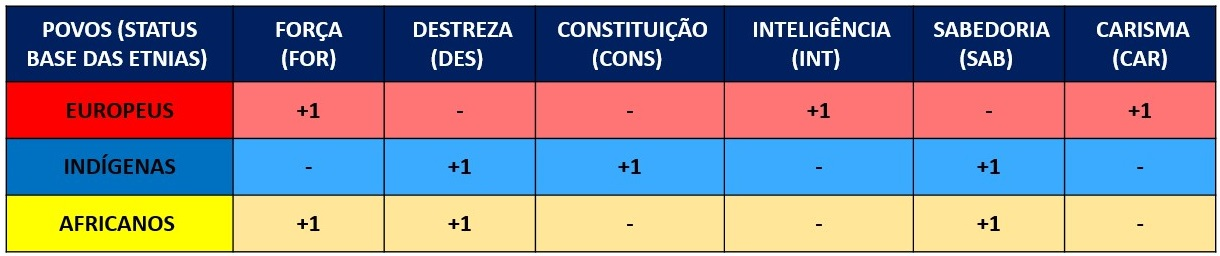
\includegraphics[width = 1.3 \CaptionWidth]{tbCriacaoPesonagem}
\SourceOrNote{Autoria Própria (2024)}
\\
\end{table}
\\
\end{itemize}

\\
\begin{table}[!h]
\centering
\SetCaptionWidth{\ifbool{@LayoutA}{0.7}{0.72}\linewidth}
\caption{Profissões}%
\label{grph:Prof}
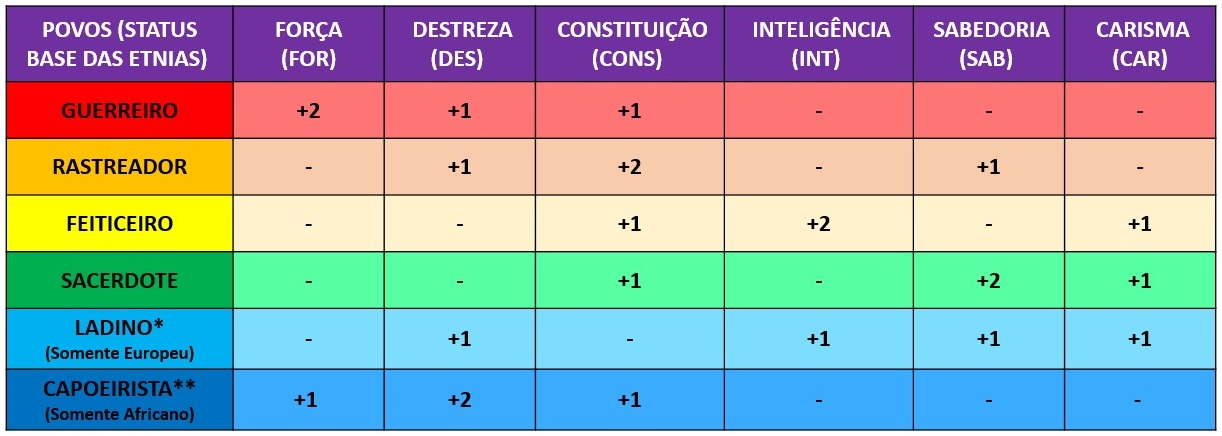
\includegraphics[width = 1.3 \CaptionWidth]{tbProfissoes}
\SourceOrNote{Autoria Própria (2024)}
\\
\end{table}
\\

As bonificações raciais concedidas pelas etnias escolhidas são aplicadas ao perfil do estudante. Após essa escolha, os estudantes poderão selecionar suas profissões, que receberão bônus específicos em seus status. A análise combinatória resulta em um total de 12 possibilidades de criação de personagens, cada um começando com 7 pontos de criação iniciais. Em seguida, o sistema concederá mais 6 pontos de bonificação, que poderão ser distribuídos conforme os estudantes desejarem, desde que nenhum atributo fique zerado ou maior que 4 no início da campanha. Durante o jogo, os estudantes terão a oportunidade de ganhar mais pontos de atributos e distribuí-los entre seus status de acordo com a orientação e o progresso no jogo. 
\\

\\
\begin{itemize}
\\
  \item \textbf{Iniciando a Campanha:} Dependendo da etnia escolhida, o sistema dará início à Campanha em uma localidade específica. Como ponto de partida, serão oferecidos escolhas e desafios aos estudantes, permitindo que escolham o caminho e percurso a seguir. O nível de dificuldade desses desafios será determinado pela análise do sistema, com base no banco de dados do Google Classroom vinculado durante o cadastro do estudante. Este banco de dados fornece um pré-diagnóstico do nível de desenvolvimento do estudante, com base na Matriz de Referência para o teste de Língua Portuguesa do SAEB para a 3ª Série do Ensino Médio (que é a mesma para o 9º Ano do Ensino Fundamental dos Anos Finais). Essa matriz é composta por seis tópicos relacionados às habilidades desenvolvidas pelos estudantes, cada um com um conjunto de descritores ligados às competências desenvolvidas. 
\\
 \item \textbf{Escolhas de Desafios:} As escolhas de desafios serão baseadas na Escala de Proficiência em Língua Portuguesa, utilizando as descrições de níveis correspondentes. Esta escala de proficiência é composta por níveis progressivos e cumulativos, o que significa que ela está organizada em níveis que vão do menor para o maior, e cada nível de desempenho acumula os conhecimentos e habilidades dos níveis anteriores. Portanto, quando um grupo de estudantes é posicionado em um determinado nível da escala, presume-se que esses estudantes tenham desenvolvido não apenas as habilidades descritas nesse nível, mas também as habilidades dos níveis anteriores. 
\\
\item \textbf{Conquitas e Evolução:} Os estudantes terão acesso a uma tela que mostrará a progressão de seus personagens, exibindo as conquistas adquiridas ao longo da jornada. Isso incluirá o avanço de nível do personagem, ganho de Pontos de Experiência (PE), obtenção de itens e benefícios após a conclusão dos desafios, bem como a capacidade de desbloquear Tokens para melhorar seus personagens. Esses dados serão transferidos para a visão do professor, permitindo que acompanhe a evolução dos estudantes e realize uma análise diagnóstica das defasagens sanadas e das dificuldades ainda presentes. Isso possibilitará o desenvolvimento e aplicação de planos de ação para realinhar a aprendizagem dos estudantes, consolidando os conhecimentos adquiridos e aprofundando aqueles que já possuíam. 
\\
\item \textbf{Período e Desenvolvimento:} Esta proposta é anual e organiza as Trilhas Pedagógicas Gamificadas em "Temporadas" distintas, cada uma composta por 4 Capítulos. O objetivo é desenvolver as habilidades, competências e conteúdos do respectivo currículo em questão, organizados por Escala de Proficiência, Level Cap (limite máximo de nível que o jogador pode alcançar durante um determinado período) e EPIC LEVEL (todos os pontos adicionais que o estudante conseguir durante o Level Cap serão convertidos ao término da Temporada em Níveis Épicos, concedendo benefícios adicionais aos jogadores).
\\
\end{itemize}

Ao fazer login no sistema, os professores terão acesso aos seguintes menus:
\\

\\
\begin{itemize}
\\
\item \textbf{Cadastro da Turma no Sistema:} O professor tem suas aulas atribuídas, e essa informação é vinculada ao seu perfil institucional na Secretaria Escolar Digital. Como o email do professor é da Google, ele tem acesso aos dados das turmas disponíveis para acompanhamento no Google Classroom. Com o email institucional, o professor se cadastra no sistema do TPG System. Isso permite o compartilhamento de informações das turmas entre os dois sistemas, garantindo a integração dos dados e facilitando o acompanhamento das atividades e evolução dos estudantes pelo professor.
\\

\item \textbf{Iniciando a Campanha e Escolhendo os Desafios:} Com base nos dados da turma, o professor seleciona o conjunto de habilidades e competências que serão trabalhados ao longo do bimestre. Ele também indica a quantidade de desafios desejados e seus níveis de dificuldade para a sala, utilizando as informações da Escala de Proficiência do SAEB. Essa escala é agrupada no SARESP em quatro níveis de proficiência (Abaixo do Básico, Básico, Adequado e Avançado), os quais são definidos a partir das expectativas de aprendizagem (conteúdos, competências e habilidades) estabelecidos para cada ano/série e disciplina no currículo do Estado de São Paulo (\Cref{grph:tabNivelProf}).
\\

\begin{table}[!h]
\centering
\SetCaptionWidth{\ifbool{@LayoutA}{0.7}{0.72}\linewidth}
\caption{Níveis de Proficiências}%
\label{grph:tabNivelProf}
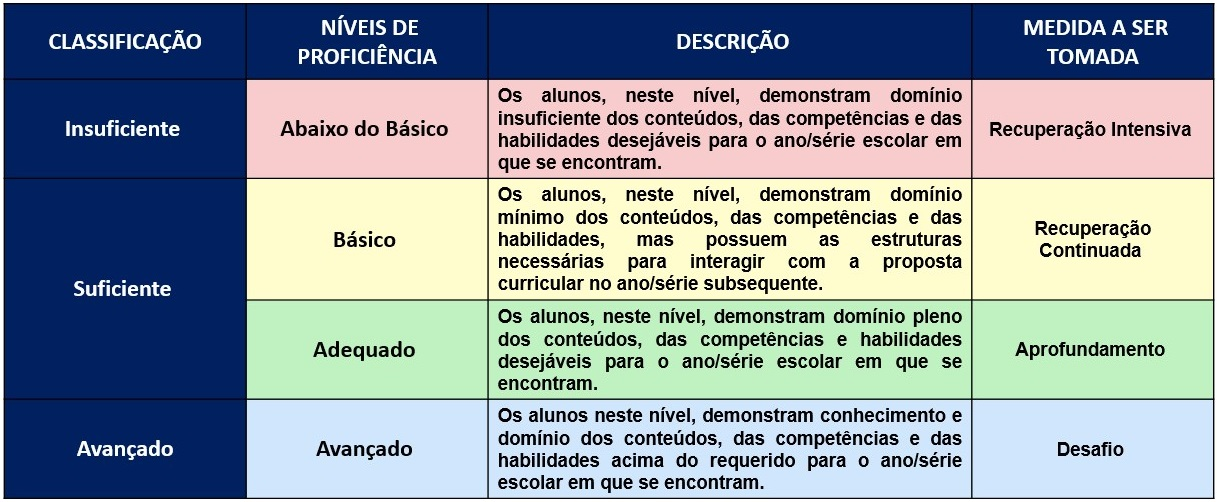
\includegraphics[width = 1.3 \CaptionWidth]{Illustrations/tbNivelProficencia.jpg}
\SourceOrNote{Elaboração própria a partir do Boletim SARESP (2022).}
\\
\end{table}
\\

\item \textbf{Conquitas e Evolução:} Através do seu perfil no TPG System, o professor terá acesso aos relatórios de evolução e conquistas dos estudantes. Ele poderá visualizar as alternativas escolhidas por eles para responder a um desafio, o tempo que levaram para concluir a atividade, bem como seus acertos e erros. Todas essas informações são cruciais para realizar o balanceamento dos resultados e autorizar as progressões e conquistas obtidas pelos estudantes. Dessa forma, o professor terá duas visões do processo evolutivo: uma dentro do jogo e outra no desenvolvimento no mundo real.
\\

\item \textbf{Período e Desenvolvimento:} Os professores, com base nos relatórios de aprendizagem disponibilizados pelo TPG System, poderão articular a aprendizagem adquirida no jogo para ser testada e validada no ambiente real, por meio de situações de aprendizagem convencionais. Isso permite que essa metodologia valide aquilo que foi desenvolvido de forma lúdica e gamificada, possibilitando que os estudantes ressignifiquem seus conhecimentos e percebam que a aprendizagem pode ser verdadeiramente impactante e transformadora. A contextualização dessas práticas com a vivência no cotidiano torna a aprendizagem integral.
\\
\end{itemize}